\documentclass[sigplan,11pt,nonacm=true,anonymous]{acmart}

\settopmatter{printfolios=false,printccs=false,printacmref=false}

\graphicspath{{assets/figures/}}

\emergencystretch=1em

\renewcommand{\_}{\textunderscore\allowbreak}

\begin{document}

\title{Measured Acceptance and Rollback as a Quality Gate for
Agent-Generated SQL}

\author{Maksim Radionov}
\affiliation{\institution{SberTech, SberData}
  \city{Moscow}\country{Russia}}
\email{radionov.maxim@gmail.com}

\author{Pavel Stepanov}
\affiliation{\institution{Unison}
  \city{Yerevan}\country{Armenia}}
\email{pstepanov@unison.team}

\author{Nikita Moskovchuk}
\affiliation{\institution{Russian University of Transport}
  \city{Moscow}\country{Russia}}
\email{1277302@edu.rut-miit.ru}

\author{Daria Lavitskaya}
\affiliation{\institution{Novosibirsk State University}
  \city{Novosibirsk}\country{Russia}}
\email{d.lavitskaya@g.nsu.ru}

\author{Andrey Balles}
\affiliation{\institution{SberTech, SberData}
  \city{Moscow}\country{Russia}}
\email{Balles.An@sber.ru}

\author{Alexandra Shumailova}
\affiliation{\institution{Bauman Moscow State Technical University}
  \city{Moscow}\country{Russia}}
\email{shumaylovaayu@student.bmstu.ru}

\renewcommand{\shortauthors}{Anonymous et al.}

\begin{abstract}
Coding agents now write code that reaches production, and there is no settled
discipline for deciding whether such code stays. This paper reports a case in
which that decision rested entirely on measurement. An agent driven by a large
language model developed a seventeen-step pipeline that turns natural-language
questions into SQL queries over relational databases. Humans designed the
surrounding harness and wrote none of the pipeline. The harness records what
every step saw and decided, scores each generated query by executing it and
comparing its rows against a reference answer, and classifies the row-level
differences, so recurring defects can be mined from run records. Every proposed
step was admitted on one criterion, its measured effect on the quality of the
emitted SQL, and steps whose gains did not survive later runs were rolled
back. The resulting
pipeline raised accuracy from 70.9\% for a
single call to the same model to 76.2\% on the development set and 81.3\% on
the private test set. Run unchanged with two other generating models, an earlier
version of the same model and a model from a different developer, the
pipeline raised both, by 3.2 and 6.7 points, so its steps capture properties
of the task rather than habits of one model. Measured acceptance and rollback is a workable quality gate for code
no human authored.
\end{abstract}

\keywords{quality gates, code generation, dynamic analysis, program
instrumentation, coding agents, text-to-SQL, large language models}

\maketitle

\section{Introduction}

Coding agents have moved from completing lines to authoring change sets. Given
a repository and an issue report, an agent edits files, runs the test suite,
and iterates until the build is green~\cite{swe-bench}, with the interface it
works through setting how far it gets~\cite{swe-agent}. Code
written this way is entering ordinary projects. The quality question that
follows is procedural. On what basis is a change written by an agent admitted
into a system, and on what basis is it taken back out?

For code covered by tests the answer is familiar. A failing test names the
behavior that broke and narrows the search for the code responsible. Other
classes of generated code have no comparable signal. Text-to-SQL is one of
them. The task is to turn a natural-language question into a query over a
relational database, and the standard measure is execution accuracy, under
which a query counts as correct only when running it returns the same rows as a
reference query~\cite{bird}. A run over the development set of the BIRD
benchmark collapses 1,534 such verdicts into one percentage. Individual wrong
answers are often noise: the query reads the question correctly and disagrees
with the reference only on a convention---an extra projected column, a
\texttt{DISTINCT} that deduplicates a fan-out join, a \texttt{NULL} in the top
row of an ordered result. The defects worth writing code against are the ones
that recur across many questions, and the aggregate hides them. A score that
fails to move reports that something is wrong without reporting which code is
wrong or why.

Two things make that gap consequential. First, generated SQL fails quietly. A
query with a wrong join or a wrong aggregation returns a table rather than an
exception, so the defect travels to whoever reads the answer. Second, the
systems that emit such queries are no longer single model calls. The strongest are
multi-stage pipelines that wrap the model in schema linking, candidate
generation, selection, and
repair~\cite{chase-sql,xiyan-sql,metadata-extraction,agentar-scale-sql}. Every
stage is a piece of code whose only justification is the quality of the queries
that come out of it. Once an agent writes those stages, a project maintains code it
did not author, aimed at defects it never enumerated, and judged by a number
that cannot be traced back to any stage.

Existing pipelines report their resulting accuracy, while autonomous
research frameworks also evaluate proposed pipeline changes~\cite{ai-scientist-enterprise}.
Our focus is how per-question and per-step records support acceptance and
later rollback of agent-written code.

We used measured acceptance and rollback to develop a text-to-SQL pipeline. Humans designed an
instrumented harness and fixed a single rule of admission. Inside it a frontier coding agent
(Claude Opus, working in Claude Code) ran the development loop: run the
benchmark, mine the recorded run for a recurring failure signature, propose a
pipeline step aimed at that signature, and measure the net effect. Humans
reviewed proposals and could inspect the selected question group, reverted the steps whose gains
did not survive later runs, and wrote none of the pipeline code. We ask three
research questions.

\begin{itemize}
\item[RQ1] Can measured acceptance and rollback act as a practical quality
  gate for pipeline code that no human wrote, admitting a step only on its
  measured effect on the SQL the pipeline emits and removing it once that
  effect stops holding?
\item[RQ2] Which quality defects of generated SQL does trace-driven error
  mining surface, and what repair code does each justify?
\item[RQ3] Does the quality of an artifact accepted under that gate transfer to
  a different generating model, or does it belong to the model it was measured
  against?
\end{itemize}

The thesis of this paper is that execution records can support acceptance
and rollback of agent-written changes:
pipeline code written entirely by an agent is fit to keep when every step has
to earn its place by a measured effect on the executed artifact and loses that
place as soon as the effect stops holding.

The 17 steps that survived the gate raise execution accuracy on BIRD's
development set from 70.9\% for a single call to the same model to 76.2\%, and
reach 81.3\% on the private test set that no part of the development loop ever
touched. The paper contributes:

\begin{itemize}
\item a quality gate for agent-written code, stated as a procedure: propose
  from a failure signature localized in run records, measure over the closed
  set of questions the change can affect, re-measure over the full question
  set, and roll the change back when a later run argues against it;
\item an instrumented harness that keeps the gate cheap enough to run
  repeatedly: every generated query is executed and scored against a reference
  answer,
  each disagreement is classified row by row, every step reports its own
  decisions, and any two runs can be compared question by question;
\item the artifact the gate produced, a pipeline of 17 steps in five groups
  (table selection, schema building, generation and review, targeted repairs,
  normalizers), each bounding its own worst case and detecting its target with
  deterministic code wherever the schema or the query's syntax supplies the
  evidence, reported with its measured quality and with a stage-level
  decomposition of the gain read off ordinary runs rather than ablation
  reruns;
\item transfer measurements with other generating models, including a
  GigaCode improvement from 59.8\% to 66.5\% on BIRD development.
\end{itemize}

\section{Related Work}
\label{sec:related-work}

\paragraph{Hand-engineered text-to-SQL pipelines.} The systems at the top of
the BIRD benchmark share a decomposed shape of schema linking, candidate
generation, selection, and repair. It descends from DIN-SQL's decomposition of
the task~\cite{din-sql} and was elaborated by CHASE-SQL and XiYan-SQL into
multi-path generation with a choice among the
candidates~\cite{chase-sql,xiyan-sql}. Automatic metadata extraction shows
that statistical profiling of a database carries much of the benefit of an
expert-written schema description~\cite{metadata-extraction}, and
Agentar-Scale-SQL orchestrates internal, sequential, and parallel test-time
scaling~\cite{agentar-scale-sql}. The pipeline reported here reuses techniques
from this line. However, every stage in these systems records a diagnosis that
a human researcher made by reading model outputs and deciding what to build
next, and what such a system publishes is the accuracy that resulted, not the
evidence behind each stage.

\paragraph{Engineering discipline inside generation pipelines.} A second line
treats the pipeline as a piece of software rather than a prompting strategy.
DeepEye-SQL imports software engineering practice into text-to-SQL through
modular stages, unit-test-style validation of candidate queries, and
systematic repair~\cite{deepeye-sql}. However, the discipline there governs
the artifact rather than the process that produced it. The architecture is
human-designed, and nothing in the method decides which pipeline code is
allowed to stay.

\paragraph{Coding agents and the gates on what they write.} A third line
studies agents that write code. SWE-bench asks whether a model can resolve
real issue reports by editing a repository until its tests
pass~\cite{swe-bench}, and SWE-agent shows that how much an agent achieves
depends on the interface it works through~\cite{swe-agent}. However, the gate
on the code these agents produce is a test suite someone else wrote or a human
reading the diff. Neither applies to a pipeline stage whose correctness is
settled by the quality of the queries emitted downstream of it.

\paragraph{Autonomous development loops for text-to-SQL}
\citet{ai-scientist-enterprise} adapt an autonomous research framework to
text-to-SQL, the framework running the loop with no human in it and
judging each proposal by the benchmark score it produces. An earlier run of
the framework, in which the executor model drew its ideas from a general
prompt, left 7 of its 10 ideas with no measurable improvement, and what
repaired the ratio was a planning stage producing granular, validated
blueprints, with the implementation model unchanged. However, the signal that governs admission is an aggregate score,
which reports that a proposal failed to help without localizing the defect it
was meant to fix.

The gate studied here differs from all four on one axis. Proposals start from
a failure signature localized in the records of a previous run rather than
from a score or a general prompt, admission is decided by a measurement over
the executed artifact rather than by a test suite or a reviewer, and rollback
belongs to the discipline, so a step leaves the pipeline once a later run
stops supporting it. To the best of our knowledge, whether measured
acceptance and rollback alone suffices as the quality gate for an entire
generation pipeline written by an agent has not been studied yet.

\section{Methodology}
\label{sec:methodology}

The experiment separated two roles. Humans designed the measuring apparatus and
fixed the rule by which pipeline code was admitted or removed. The agent
designed and implemented every step of the pipeline that turned a question into
SQL. The agent analyzed the run traces. Humans could inspect a selected group
of questions in detail before a full development run.

\begin{figure}[t]
  \centering
  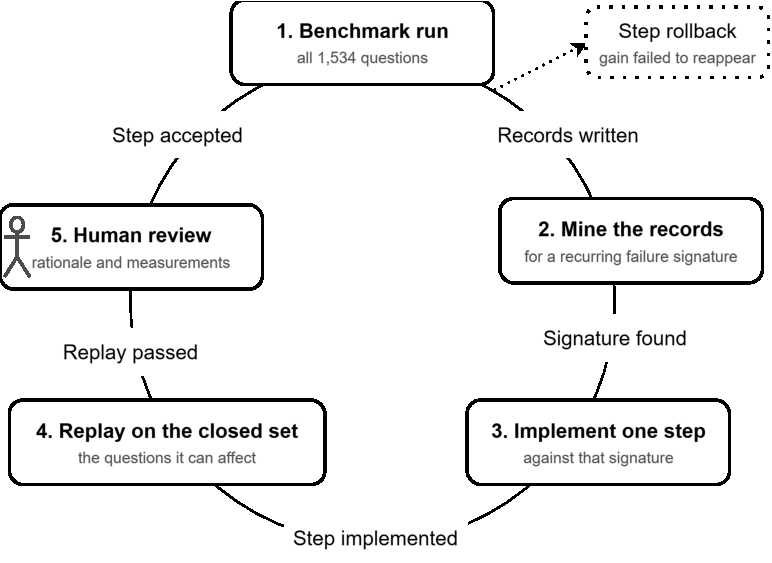
\includegraphics[width=\columnwidth]{harness_iccq-fig}
  \caption{The harness and the development cycle inside it. A full benchmark
  run leaves records; the agent mines them for a recurring failure signature,
  implements one step against it, and replays the change over the closed set
  of questions it can affect. Human review admits the step into the next
  pipeline version, whose full run measures the combined effect, and a later
  run that argues against a step removes it.}
  \label{fig:harness}
\end{figure}

\paragraph{The harness.} A single command ran a named pipeline version over a
question set and produced the entire record of that run
(Figure~\ref{fig:harness}). On disk, a timestamped
directory held the fully resolved configuration, pinning the pipeline version,
the models, and the question subset. Beside it grew an append-only predictions
file with one record per question, carrying the question and its evidence hint,
the reference and generated SQL, the rows each of them returned, and the
verdict. A run log and a diff report over every miss completed the directory.
The same execution was mirrored as a telemetry stream into a local Arize
Phoenix instance,\footnote{\url{https://docs.arize.com/phoenix}} one span per
step recording its kind, its duration, what it
saw and what it decided, and, for model calls, the prompt, the response, and
the tokens they cost. Every run registered itself as an experiment against a
question set pinned as a dataset, so any two runs could be aligned question by
question.

\paragraph{Scoring.} The harness judged an answer by running it. It executed
both the generated query and the reference query against the database and
compared the two sets of result rows as unordered sets, the local execution-accuracy measure used for accept-or-revert decisions. Scoring in this form is dynamic analysis
over the generated artifact: nothing is inferred from how a query reads, and
the verdict comes from what it returns on a real database.

\paragraph{Classifying disagreements.} A wrong answer was decomposed rather
than counted. For each question the predictions file named the rows missing
from the generated result and the rows that should not have been there. The
diff report paired reference and generated rows side by side and sorted each
mismatching value into one of three kinds: the same number written in a
different format, two date-like values, or genuinely different
values. A miss therefore stated in what way it was wrong, in text that could be
grepped and clustered across a run.

\paragraph{Step self-reporting.} Every step reported on itself. The runner
contributed only the step's kind and its timing to the span, while the account
of what the step received and what it decided came from the step's own code and
was written to the run log as well. Adding a step meant following that
convention, so the agent's own additions arrived instrumented, and the next run
already showed how often a new step fired, on what evidence, and what it
changed. Clustering those records over a run is what localized a defect,
tracing a signature that recurred across many questions to the step that
produced it or should have caught it. Such localization is statistical over a
corpus rather than exact over one failing execution---a weaker instrument than
a failing test and a much stronger one than an aggregate score.

\paragraph{The documented interface.} One instruction file in the agent's
working environment described the mechanics: the command that started a run,
the artifacts it left and where they lived, how to query the telemetry store,
and how to add a step. The file covered measurement discipline and nothing
else. It named no text-to-SQL technique, diagnosed no failure, and proposed no
step.

\paragraph{The development cycle.} The agent was Claude Opus, versions 4.6
through 4.8 as they became available over the course of the project, working
in Claude Code.
One turn of the loop (Figure~\ref{fig:harness}) began with a full run over the
development set. The agent
read its records until a failure signature recurred across enough questions to
warrant code, then implemented one step aimed at that signature, with
self-reporting included, and replayed the modified pipeline over the closed set
of questions the change could affect: the failures that motivated it, together
with the passing questions it could plausibly break. A step that repaired its
targets and left its neighbors intact was bundled with the other accepted
changes into the next named pipeline version, and that version ran over all
1,534 development questions. Comparing the two versions question by question
reported how many answers had been gained and how many lost.

Before a full run, proposals were screened for a target group of at least
ten questions, to avoid spending tokens on changes with too little expected
reach; this was not a requirement of ten net corrections after execution.

\paragraph{Human review and rollback.} Humans reviewed the rationale of each
proposed step together with the measurements attached to it, and wrote none of
the pipeline code. Acceptance was provisional. At least seven changes cleared review and
their replay test only to be removed later, when the gains that had justified
them failed to reappear in subsequent full runs. In the clearest case a cluster
of challenging misses shared one cause---a reference query routing through a
bridge table the generated query never joined. The step the agent wrote against
it closed foreign-key paths across bridge tables and ran in three full
benchmark runs. The same questions stayed wrong in all three, and the step was
removed.

\paragraph{The gate.} Stated as a procedure, admission imposed four
requirements. A
change had to originate in a defect signature already localized in the records
of a completed run, not in a hypothesis about the task. It had to be measured
first over the closed set of questions it could touch, where its repairs and
its collateral damage were visible at once. It then had to be re-measured over
the full question set inside a named pipeline version, competing there with
everything else that version carried. And it stayed removable, so a later run
arguing against a step took the step out regardless of the measurement that had
first admitted it. Nothing else counted: neither the plausibility of a
rationale nor a reviewer's opinion of the code could admit a step on its own.

\section{Pipeline}
\label{sec:pipeline}

The pipeline described here is the last of a series. Its first version predated
any observed failure: humans handed the agent two papers, on statistical schema
profiling~\cite{metadata-extraction} and on agentic data
exploration~\cite{apex-sql}, neither with a public implementation at the time,
and the agent reproduced both from the text alone. Later versions grew inside
the loop of Section~\ref{sec:methodology}, within which the agent chose its own
reading and consulted the systems at the top of the BIRD
leaderboard~\cite{bird-leaderboard} when a failure pointed at an established
technique. The seed was not exempt from the gate: the profiling half is still
in the pipeline below, and the exploration half was scored out by a later full
run.

Seventeen steps survived, in a fixed order, in five groups
(Figure~\ref{fig:steps}): three for table selection,
five for schema building, two for generation and review, four targeted
repairs, and three normalizers. A step receives the question, its evidence
hint, and everything the earlier steps recorded, and it either extends that
context or rewrites the query.

\begin{figure*}[t]
  \centering
  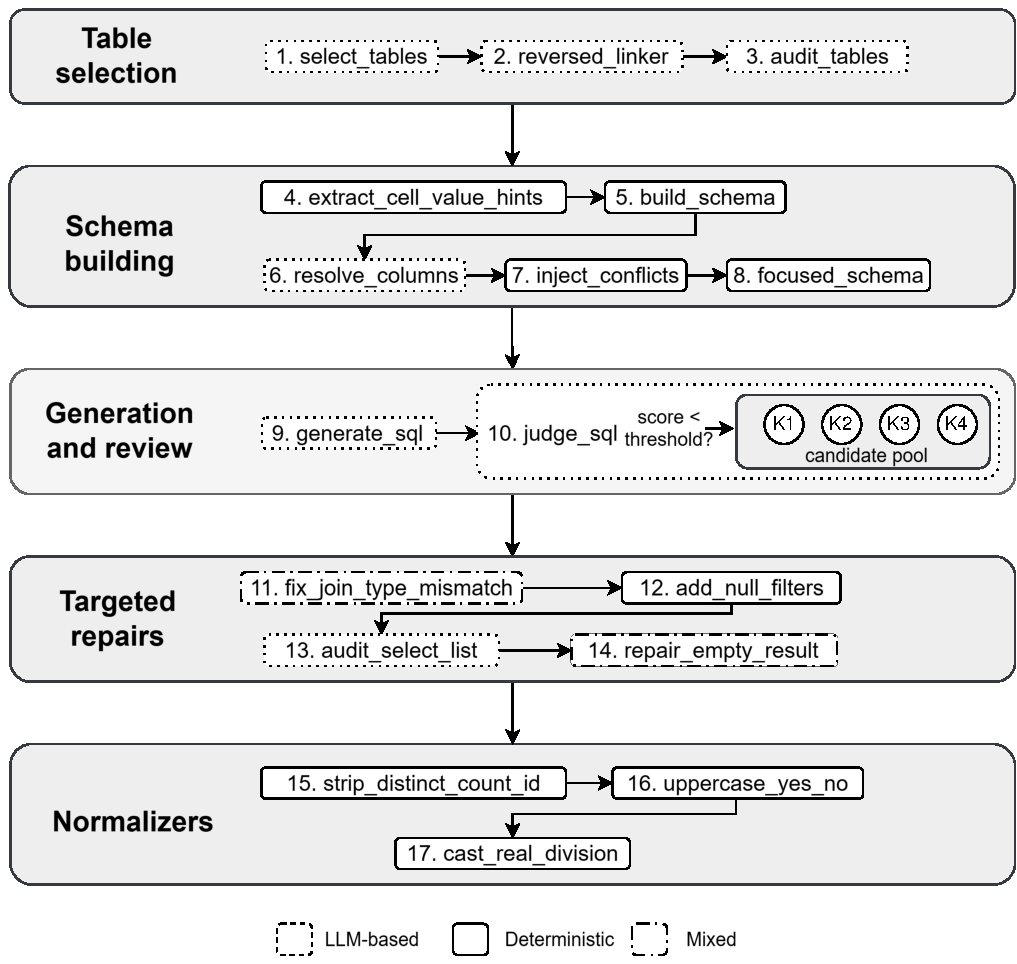
\includegraphics[width=0.78\textwidth]{steps_iccq-fig}
  \caption{The 17 steps as data flow, named by their identifiers in the
  pipeline source and grouped by function. The border style marks how a step
decides:
  by a call to a language model, by deterministic code, or by a mix in
  which deterministic code detects the defect, a language model drafts the
  rewrite, and a deterministic check accepts or discards it. Context
  accumulates until generation, and every step after it either passes the
  query through untouched or rewrites it behind its guards.}
  \label{fig:steps}
\end{figure*}

\paragraph{The shared conservative design.} What makes a chain of seventeen
rewrites viable is a shared conservative design. Each step is an opportunity to
break a query that was already correct, and the opportunities compound unless
every step passes a correct query through untouched. Four properties do that
work. Each step bounds the worst case it can produce and keeps that bound
small. Each fires only on positive evidence, so a query with no symptom leaves
a step exactly as it arrived. Detection is deterministic wherever the schema or
the syntax of the query supplies the evidence. And where a model call is
involved, it drafts the rewrite but never decides whether the rewrite is kept:
a check on the rewritten query accepts it or restores the query the step
received. The gate selected this design rather than prescribing it. An unguarded
rewrite repairs the questions it was written for and breaks others it never
considered, so its net effect over 1,534 questions comes out small or negative
and the step does not survive.

\paragraph{Table selection.} Three model calls narrow the database to the
tables a question needs. \texttt{select\_tables} proposes a set from a profile
computed once per database~\cite{metadata-extraction}: row counts, NULL rates,
numeric ranges, and value distributions, with low-cardinality columns
enumerated in full. Those statistics make the later choices value-grounded, so
a literal in the question can be matched against a column's actual domain
rather than against its name. \texttt{reversed\_linker} works
backwards~\cite{deepeye-sql}: instead of asking for a list of tables, it asks
for a draft query over the full catalog, discards the draft, and keeps the
tables the draft referenced, which recovers the bridge tables a name-matching
selector misses.
\texttt{audit\_tables} asks once whether anything relevant is still missing.
All three are recall-biased for the same reason: a missing table cannot be
recovered downstream, while an extra one costs tokens. The worst case is
bounded by monotonicity: the two steps after the selector can only add tables
to its set, and a failure inside the selector falls back to every table in
the database.

\paragraph{Schema building.} Five steps turn the selected tables into the text
the generator reads. \texttt{extract\_cell\_value\_hints} scans the question
for phrases stored verbatim as cell values and records the table and column
where each one lives~\cite{deepeye-sql}. \texttt{build\_schema} renders the
selected tables as an extended M-Schema~\cite{xiyan-sql} carrying the same
profiling statistics, and every step downstream reads the database through that
rendering. \texttt{resolve\_columns} binds each concept in the question to
exactly one column and must list the plausible alternatives it rejected as
conflicts. That binding is a contract downstream, and the run records exposed
its failure mode: a concept bound to a look-alike with an empty conflict list
freezes the error, because the generator never sees the column it should have
chosen instead. \texttt{inject\_conflicts} reopens those cases, retrieving
look-alikes by name overlap and embedding rank~\cite{qwen3-embedding} for every
concept the previous step left conflict-free. In the final run it added
conflict sets to 1,201 of the 1,534 questions, 2,227 concepts in all.
\texttt{focused\_schema} trims the rendering down to the resolved columns,
their conflicts, and every key, so the join paths survive. The trim is where
the group's worst case is bounded: it may not drop a column that either of
the two binding steps put in play, so every resolved column reaches the
generator.

\paragraph{Generation and review.} \texttt{generate\_sql} turns the question,
the evidence hint, the focused schema, the column bindings, and the cell-value
hints into a query in one call to the strongest available model. A query that
executes and returns zero rows counts as a failure and triggers one
regeneration. No reference answer on the development set is empty, so a
valid-but-empty result is always wrong. \texttt{judge\_sql} then scores the
query. At or above a threshold the pipeline spends nothing further on review.
Below it, the step assembles a pool of four candidates: the original, a
corrective rewrite of it, a variant generated with explicit reasoning, and a
variant generated from a decomposition of the question. Candidates whose result
rows are identical collapse into one, and a winner is chosen by pairwise
votes~\cite{agentar-scale-sql}, with every tie and every unparsable vote
resolving toward the original. The threshold is what makes the pool affordable.
In the final run it opened on 118 of the 1,534 questions.

\paragraph{Targeted repairs.} Four steps each own one defect signature that
kept recurring in the run records. \texttt{fix\_join\_type\_mismatch} parses
the query and compares the declared types of the columns each join equates. A
join across an INTEGER key and a TEXT key is detected from the schema alone, a
model drafts the rewrite, and the rewrite is kept only if the mismatch is gone
and rows come back. \texttt{add\_null\_filters} guards an \texttt{ORDER
BY \dots{} LIMIT} whose top row carries a NULL sort key---a shape that returns
a row answering nothing. \texttt{audit\_select\_list} is confined to the
projection, where it repairs a look-alike column, a plural question answered
with a single column, or one field too many. It may touch nothing else, and it
answered OK on 1,515 of the 1,534 questions of the final run.
\texttt{repair\_empty\_result} is the backstop for the empty-result symptom:
read-only probes establish why the result is empty, a model drafts a rewrite
from what they found, and the step discards about half of those drafts on its
own validity checks. Its position is load-bearing. It runs last among the steps
that can change which rows come back, because an earlier arrangement let
\texttt{audit\_select\_list} run afterwards and revert a repaired query to
empty. Two of these four did not fire once across the final run, their
signatures squeezed out upstream as selection and generation improved. Both
stay, since detection is deterministic and an idle pass costs nothing.

\paragraph{Normalizers.} Three deterministic passes over the parsed query close
the pipeline, and none changes which rows the query returns.
\texttt{strip\_distinct\_count\_id} removes \texttt{DISTINCT} from counts over
identifier columns, \texttt{uppercase\_yes\_no} raises lowercase yes and no
literals to the casing the reference answers use, and
\texttt{cast\_real\_division} inserts a cast where a projection divides one
integer by another. Every join and every filter passes through untouched, which
is what licenses running these three after the backstop. What they rewrite is
how the answer is expressed: whether a count deduplicates, how a literal is
cased, whether a division truncates. When results are compared as sets of
rows, those details alone separate a right answer from a wrong one, so a
rewrite there can flip a verdict in either direction.

\paragraph{One step in detail.} \texttt{strip\_distinct\_count\_id} shows what
the guards are worth. Asked how many X there are, the model defensively writes
\texttt{COUNT(DISTINCT id)} where the reference query counts joined rows as
they come, and the two answers diverge exactly when a join fans out. Three of
the step's four guards are simple: the question must not itself ask for
distinctness, every counted column must be identifier-shaped, and the stripped
query must still execute. The fourth is a confidence gate on the judge's score,
calibrated by replaying the strip against the recorded results of all 1,534
development questions and sweeping the cutoff, which shows for every candidate
value which questions it repairs and which it breaks. The chosen value sits in
the middle of the band the sweep marked safe, away from the edge where the
strip starts breaking correct answers. In the final run 89 queries reached the
step carrying a \texttt{COUNT(DISTINCT \dots{})} and 51 were rewritten, the
step standing down on 21 whose question asked for distinctness, 8 counting a
column that was not identifier-shaped, and 9 the judge had endorsed above the
gate.

Read against RQ2, every step after generation descends from a defect signature
the run records made legible and some check could then recognize. A query that
executes to zero rows, on a benchmark where no reference answer is empty,
licenses \texttt{repair\_empty\_result}. A concept bound to a look-alike with
no alternative recorded licenses \texttt{inject\_conflicts}. A defensive
\texttt{COUNT(DISTINCT \dots{})} over an identifier column licenses
\texttt{strip\_distinct\_count\_id}. A join equating columns of different
declared type licenses \texttt{fix\_join\_type\_mismatch}. Every pair is the
same move: a defect visible in the records became a predicate, and the
predicate became the guard on a rewrite. Defects the records exposed but no
predicate could recognize produced no step at all.

\section{Experiments}

All development ran against the development set of BIRD~\cite{bird}, 1,534
questions that the benchmark splits into 925 simple, 464 moderate, and 145
challenging. The test set is private, and no part of the development loop
touched it. Quality is reported as execution accuracy, scored exactly as every
gate decision was scored (Section~\ref{sec:methodology}): a prediction counts
as correct when the rows it returns, compared as a set, agree with the rows of
the reference query.

Three generating models appear in the measurements. Claude Opus~4.8 is the
model the pipeline was developed against, and every acceptance and rollback
decision was measured on it. Claude Opus~4.6 is an earlier version of the same
model. GigaCode~1.6 comes from a different model family and a different
developer. Each model appears in two configurations. Single-shot issues
one call carrying the instructions, the database schema, and the question, and
takes the returned query as the answer. Agent-built runs the 17-step pipeline
that the quality gate admitted. Table~\ref{tab:results} reports the six
configurations.

\begin{table}[t]
\caption{Execution accuracy (EX, \%) on BIRD by difficulty tier. Single-shot is
one call to the model, carrying the instructions, the database schema, and the
question. Agent-built is the 17-step pipeline the quality gate produced, run
unchanged on all three models. A dash marks a score that was not
measured.}
\label{tab:results}
\centering
\footnotesize
\setlength{\tabcolsep}{4pt}
\begin{tabular}{@{}lrrrrr@{}}
\toprule
Configuration & Simp. & Mod. & Chall. & Dev & Test \\
\midrule
\multicolumn{6}{@{}l}{Claude Opus 4.6} \\
\quad single-shot & --- & --- & --- & 68.8\rlap{$^*$} & 70.2\rlap{$^*$} \\
\quad agent-built & 77.1 & 64.7 & 62.8 & 72.0 & --- \\
\addlinespace[2pt]
\multicolumn{6}{@{}l}{Claude Opus 4.8} \\
\quad single-shot & 75.0 & 64.7 & 64.8 & 70.9 & --- \\
\quad agent-built & 80.7 & 72.0 & 61.4 & 76.2 & 81.3\rlap{$^\dagger$} \\
\addlinespace[2pt]
\multicolumn{6}{@{}l}{GigaCode 1.6} \\
\quad single-shot & 66.2 & 52.2 & 43.4 & 59.8 & --- \\
\quad agent-built & 73.5 & 56.9 & 52.4 & 66.5 & --- \\
\bottomrule
\end{tabular}

\smallskip
\begin{minipage}{\columnwidth}
\footnotesize\raggedright
$^*$\,Official BIRD leaderboard baseline for Claude Opus~4.6, quoted
from~\cite{bird-leaderboard}.\\
$^\dagger$\,Our submission, scored by the BIRD team on the private test set
and listed on the leaderboard~\cite{bird-leaderboard}.
\end{minipage}
\end{table}

The comparison that answers RQ1 is the same-model pair. One call to Claude
Opus~4.8 scores 70.9 on the development set, and the pipeline of steps admitted
by the gate, built around that same model, scores 76.2. The model is identical
in both rows, so the 5.3 points come from the context the pipeline builds for
the model and from the repairs it applies to the query the model returns. Seventeen steps written
by an agent and admitted on measured effect alone compose into an artifact that
is better than the model called directly.

RQ3 asks whether that quality belongs to the model it was measured against.
Re-run with no step changed, the pipeline lifts Claude Opus~4.6 from 68.8 to
72.0, a gain of 3.2 points, and GigaCode~1.6 from 59.8 to 66.5, a gain of 6.7.
The gain reproduces on all three models and spans 3.2 to 6.7 points, and it
does not track the strength of the base model: the largest gain belongs to the
weakest of the three, and the cross-vendor model gains more than the earlier
version of the model the steps were tuned on. Both transfer measurements are
development-set measurements, since the test set was submitted only for the
model the pipeline was developed against. There the agent-built pipeline scores
81.3---third on the BIRD leaderboard as of August 2026 and 0.6 points off
first place~\cite{bird-leaderboard}---which is external evidence that the
accepted artifact holds up on questions that no development decision could have
been fitted to. The single-shot baseline also rises between the two sets, by 1.4
points on Claude Opus~4.6, so part of the difference between 76.2 and 81.3
belongs to the question sets rather than to the pipeline.

RQ2 asks which defects the mining surfaced and what each repair is worth. The
answer is read off ordinary runs. Because every step records what it received
and what it returned, the run that scores 76.2 can be decomposed after the fact
without a single ablation rerun. From the 51,706 recorded step spans of that
run, each question's query was reconstructed at every stage of the chain,
executed against its database, and compared with the reference by the same
comparator the run itself used, 3,013 distinct executions in total. A step
\emph{saved} a question when the query entering it was wrong and the query
leaving it was right, and \emph{broke} the question in the reverse case. The
effect is local to the step's position in the chain, so one question can be
saved by one step and broken by another, which happened four times. As a
consistency check, the recomputed final verdicts agree with the verdicts
recorded by the run on all 1,532 questions the reconstruction could
re-execute.

\begin{table}[t]
\caption{Contribution of each step that rewrites the query, reconstructed from
the recorded inputs and outputs of one ordinary run: Claude Opus~4.8 with the
agent-built pipeline, the 76.2\% row of Table~\ref{tab:results}. Fired counts
the questions whose query the step rewrote, saved and broke count the rewrites
that turned a wrong answer right and a right answer wrong, and net is their
difference. Step~9 sets the baseline of 1,137 correct answers out of 1,534.
Steps~1--8 do not touch the query and admit no per-question attribution.}
\label{tab:contrib}
\centering
\footnotesize
\setlength{\tabcolsep}{3pt}
\begin{tabular}{@{}rlrrrr@{}}
\toprule
\# & Step & Fired & Saved & Broke & Net \\
\midrule
9 & \texttt{generate\_sql} & 1,534 & --- & --- & --- \\
10 & \texttt{judge\_sql} & 46 & 13 & 6 & $+7$ \\
11 & \texttt{fix\_join\_type\_mismatch} & 0 & 0 & 0 & 0 \\
12 & \texttt{add\_null\_filters} & 0 & 0 & 0 & 0 \\
13 & \texttt{audit\_select\_list} & 11 & 3 & 3 & 0 \\
14 & \texttt{repair\_empty\_result} & 6 & 4 & 0 & $+4$ \\
15 & \texttt{strip\_distinct\_count\_id} & 51 & 25 & 8 & $+17$ \\
16 & \texttt{uppercase\_yes\_no} & 3 & 1 & 0 & $+1$ \\
17 & \texttt{cast\_real\_division} & 27 & 4 & 1 & $+3$ \\
\midrule
\multicolumn{5}{@{}l}{Net after generation} & $+32$ \\
\bottomrule
\end{tabular}
\end{table}

Table~\ref{tab:contrib} reports the steps that rewrite the query. The eight
steps before generation prepare the generator's input and never edit a query, so the
table omits them and their activity is reported here: table selection, schema
building, column resolution, and schema focusing run on all 1,534 questions,
cell-value hints are found on 867, conflicting-concept annotations are injected
into 1,201, the reversed linker adds tables on 16, and the table auditor
expands a selection once. Of the total gain of 5.3 points over single-shot
generation, 3.2 are already present when the generator returns its query, which
is correct on 1,137 questions or 74.1\%, and the remaining 2.1 points are the
net $+32$ answers added by the steps that check and repair that query. More
than half of those 32 come from one step---the removal of a \texttt{DISTINCT}
inside a count over a key column---which is a database-specific counting
convention rather than a reasoning failure. The judge opened its candidate
pool on 118 questions and rewrote 46 of them. It nets $+7$ but works noisily:
only 19 of the 46 rewrites changed a verdict, 13 for the better and 6 for the
worse, and 22 replaced one wrong query with another. The two steps that never fire found nothing to repair
across all 1,534 questions, because the failures that motivated them are
prevented earlier in the chain in this version of the pipeline.

Sliced by difficulty, the gain is uneven. Against the
single-shot baseline on Claude Opus~4.8, the pipeline adds 5.6 points on simple
questions and 7.3 on moderate ones, and loses 3.4 on challenging ones, from
64.8 to 61.4. Across all Claude Opus configurations in
Table~\ref{tab:results} the challenging tier stays between 61 and 65, whether
the query comes from one call or from the pipeline. We read all 56 challenging
misses of the final run by hand. In most of them the prediction is a
defensible reading of the question that differs from the reference only in
which columns it projects or in which quantity it counts, in several the
reference contradicts the evidence hint attached to the question, and a
minority are outright reasoning errors. No rewrite aimed at any of these
classes survived measurement. What the gate harvests, on this model, are
convention-level defects that recur across many questions, and those are
concentrated in the simple and moderate tiers. The challenging tier is not
inert everywhere. On GigaCode~1.6 the pipeline adds 9.0 points there, from 43.4
to 52.4, more than it adds on simple questions (7.4) or moderate ones (4.7). A
tier that does not move for a strong model moves for a weaker one, which places
the ceiling with the model rather than with the pipeline.

\section{Practical Recommendations}
\label{sec:impact}

Reproducing this discipline does not require the pipeline of
Section~\ref{sec:pipeline}. It requires the apparatus, the rule, and a task
whose output can be run.

\paragraph{The instrumentation was ordinary.} Nothing in the harness of
Section~\ref{sec:methodology} is a research contribution in its own right. One
command runs a named pipeline version over a chosen question set. One
append-only file keeps a record per question. A convention obliges every step
to report what it received and what it decided, so code added later arrives
instrumented. A trace store holds the spans, and each run registers itself
against a pinned question set so that any two runs align question by question.
Each of those pieces is standard engineering practice, which is the point: no
analysis technique had to be invented before the gate could
operate. One property did matter: the record is kept per question and per
step, not per run. A script that reports only the final percentage cannot
support the gate, because localizing a defect and deciding a rollback both
need to know which questions changed and how. The upgrade is small, though.
Such a script already computes a verdict for every question before averaging
them into one number; keeping those verdicts, and obliging each step to log
what it received and decided, is most of what this harness is.

\paragraph{The gate transfers on three conditions.} Stated as a procedure, the
gate names nothing specific to SQL. It needs an output that can be executed
and not merely read, a reference for each item so that the executed result
can be scored item by item, and a way to enumerate in advance the items a
change can affect, so the change is replayed over that closed set before it
competes inside a full run. Rollback then follows from the same records,
because two runs scored item by item can be differenced. A generator of code
judged by tests, or of data transformations judged against expected outputs,
satisfies those conditions as stated. No such task was run through the gate
here, and Section~\ref{sec:limitations} owns that.

\paragraph{Decompose from records, not from reruns.} Because every step
recorded its input and its output, the stage-level attribution in
Table~\ref{tab:contrib} was reconstructed from one ordinary run instead of a
series of ablation reruns, each of which would have cost a full pass over the
question set. A team that keeps the self-reporting convention gets that
decomposition for the price of storage, and gets it for runs it has already
made, not only for experiments it thought to design. The limit is
visible in the same table. Steps that prepare context rather than rewrite the
artifact cannot be attributed this way, and only their activity can be counted.

\paragraph{Adopt the guarded shape rather than rediscovering it.} The gate
selected the conservative design of Section~\ref{sec:pipeline} instead of
prescribing it, because an unguarded rewrite repairs its targets and breaks
neighbors it never considered, and its net effect over a large question set
comes out small or negative. A team need not spend runs relearning that. Make
it the convention for new steps that a step fires only on positive evidence of
a defect and restores what it received whenever its own check is not satisfied,
so that measurement decides only the question that remains open---whether the
step is worth having at all.

\paragraph{Where this pays, and where it does not.} The gate harvests defects
that recur at the level of convention across many items and that some check can
recognize once the records make them legible. Where a corpus carries such
defects and the artifact can be run, they are found without anyone enumerating
them in advance. Where the corpus carries no such defects, the gate admits
nothing.
Defects the records exposed but no predicate could recognize produced no step
at all, and the difficulty tiers of Table~\ref{tab:results} show that what
remains is limited by the generating model, not by the pipeline around it. In
the division of labor that emerged, the agent supplied volume and patience,
reading every record, proposing a step against each signature that recurred,
and instrumenting what it wrote, while the measurement supplied the judgment
about what to keep.

\section{Limitations}
\label{sec:limitations}

\paragraph{Three factors acted together and cannot be apportioned.} Every step
was proposed by a frontier model, reviewed by a human, and admitted on a
measurement, and nothing in the experiment removes one of the three while
holding the others fixed. A model trained on defensive code may propose guarded
rewrites out of its training prior rather than because the gate rewards them,
and the
reviewers leaned the same way. Two facts argue that measurement was not merely
ratifying the other two. All three acted through one channel---the measured
net effect---and rollback removed at least seven changes that review had
already accepted. Neither fact is a decomposition. How much of the quality of the 17
steps belongs to the gate rather than to the model prior or to the reviewers is
not measured here.

\paragraph{One task.} Development used BIRD~\cite{bird}; transfer was also
evaluated on SQLite tasks in Spider2-Lite. Section~\ref{sec:impact} states the
conditions the gate needs in terms other generation tasks satisfy, but no other
task was put through it, so that transfer is argued and not measured. Part of
what survived is narrower than the task. Stripping \texttt{DISTINCT} from
counts over identifiers, normalizing the casing of yes and no literals, casting
an integer division, and regenerating on an empty result encode conventions of this
benchmark's reference queries, and on a corpus with other conventions those
steps would have to be earned again or dropped.

\paragraph{The agent did not build its own instrument.} Humans designed the
harness before the loop started, so the claim concerns what an agent does
inside a measurement discipline, not what it does in establishing one. The
obvious objection is that an agent writes code and could have instrumented the
benchmark itself. That experiment was not run, and nothing here rules it out.
\paragraph{The development set was measured many times.} Every acceptance and
every rollback rested on runs over the same 1,534 questions, which is sustained
pressure to fit that set. The private test result provides evidence on questions unavailable during
development; the difference between test and development scores also depends
on the question sets.
The judge's cutoff and the confidence gate on the \texttt{DISTINCT} strip were
calibrated by sweeping development-set records produced by Claude Opus, and
whether those values suit another generating model was not tested.

\paragraph{Cross-model transfer was measured on BIRD development.} The private test
column of Table~\ref{tab:results} is filled for the agent-built pipeline on one
model, the model it was developed against. The other-model results are development-set measurements,
so cross-model generalization to unseen questions remains unmeasured.

\section{Conclusion}

This paper reported an experiment in which pipeline code that no human wrote
was evaluated through measured acceptance and rollback. Humans designed an instrumented harness and
fixed one rule of admission. Inside it, a coding agent mined each completed run
for a defect signature that recurred, wrote one step against it, and measured
the result over the questions that step could touch and then over the whole
development set. Steps whose gains stopped reappearing were taken back out.

RQ1 asked how measured acceptance and rollback acted as a quality gate
for code no human authored. The records supported acceptance and later reversal. The 17 steps the gate admitted
raised the same generating model from a single-shot 70.9\% to 76.2\% execution
accuracy on the development set of BIRD and reached 81.3\% on the private test
set, and the
same rule that admitted a step removed it once a later run stopped supporting
it. RQ2 asked what trace-driven mining surfaces and what it justifies. It
surfaced defects that recur at the level of convention, each of which became a
predicate that recognized its target and guarded a rewrite: a query executing
to no rows, a concept bound to a look-alike column, a deduplicating count over an
identifier. Defects no predicate could recognize produced no step.
RQ3 asked whether the resulting quality belongs to the model it was measured
against. It does not. With GigaCode, the pipeline raised development accuracy from 59.8\% to
66.5\%.

Acceptance remained provisional throughout development. Every step earned its place by its measured effect on the executed
artifact, and no step kept a place the later measurements stopped supporting.


\bibliographystyle{ACM-Reference-Format}
\bibliography{refs/references}

\end{document}
